\normaltrue \difficilefalse \tdifficilefalse
\correctionfalse

%\UPSTIidClasse{11} % 11 sup, 12 spé
%\newcommand{\UPSTIidClasse}{11}

\exer{Identification $\star$ \label{B2:06:504}}
\setcounter{question}{0}\UPSTIcompetence[2]{B2-06}
\index{Compétence B2-06}
\index{Identification}
\index{Identification Bode}
\index{Identification fréquentielle}
\index{Réponse fréquentielle}

\ifcorrection
\else
\marginnote{\textbf{Pas de corrigé pour cet exercice.}}
\fi


\ifprof 
\else
\begin{flushright}
D'après Florestan Mathurin.
\end{flushright}

Le diagramme temporel ci-dessous présente 3 signaux d'entrée sinusoïdaux.
\begin{center}
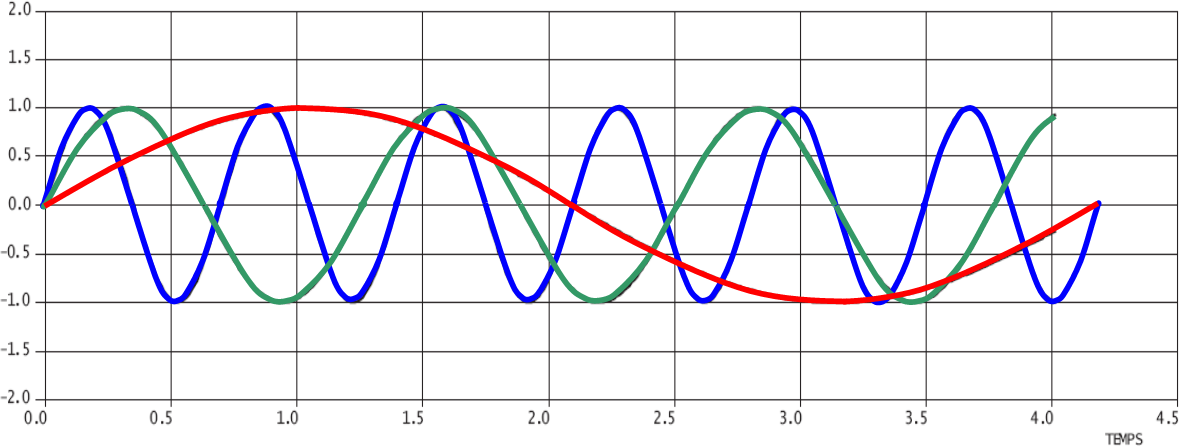
\includegraphics[width=\linewidth]{504_01}
\end{center}
\fi

\question{Déterminer les période et les pulsations de chacun des signaux.}
\ifprof
\else
\fi


\question{En déduire le gain et le déphasage en régime permanent pour chacune des courbes temporelles de sortie correspondant aux 3 entrées.}
\ifprof
\else
\fi




\ifprof
\else
\begin{flushright}
\footnotesize{Corrigé  voir \ref{B2:06:504}.}
\end{flushright}%
\fi